\chapter{Resultados}

Tras probar diferentes ajustes he detectado que había `sobreaprendizaje', esto es que aunque se mejora mucho el resultado para el conjunto de entrenamiento, a la hora de aplicar lo aprendido sobre el conjunto de prueba diera malos resultados. Tras ir ajustando los parámetros de las diferentes capas añadidas así como el número de neuronas se ha alcanzado una solución que daba unos resultados mas similares entre ambos conjuntos, siendo por tanto esta solución mucho mejor que un resultado dispar.

\bigskip
Los resultados obtenidos tras diversos ajustes en el algoritmo son bastante buenos, pasamos a detallarlos:

\begin{table}[H]
\centering

\begin{tabular}{|l|r|}
\hline
Tiempo de entrenamiento (en segundos)                 & 187  \\ \hline
Tasa de error sobre el conjunto de entrenamiento (\%) & 0.05  \\ \hline
Precisión sobre el conjunto de entrenamiento (\%)     & 99.95 \\ \hline
Tasa de error sobre el conjunto de prueba (\%)        & 0.64  \\ \hline
Precisión sobre el conjunto de prueba (\%)            & 99.36 \\ \hline
\end{tabular}
\caption{Tabla de resultados}

\end{table}

En la figura \ref{fig:plot} podemos ver como ha ido bajando el porcentaje de error en cada lote.

\begin{figure}[H]
\centering
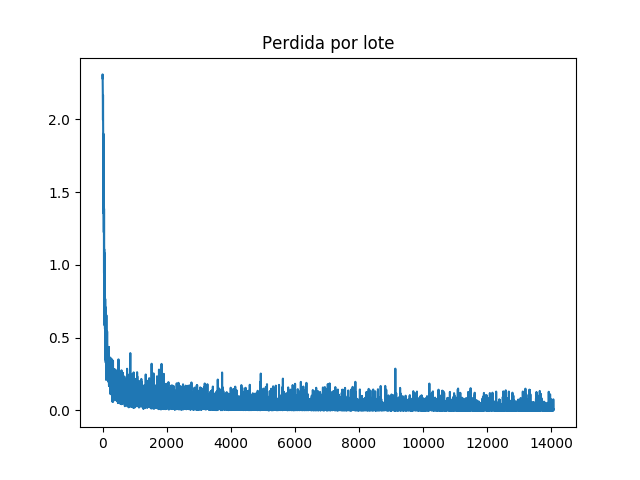
\includegraphics[width=1.0\textwidth]{../images/plot}
\label{fig:plot}
\end{figure}


